\section{Jawna metoda dwustopniowa (ulepszona Eulera)}
%%%%%%%%%%%%%%%%%%%%%
\begin{frame}{Etap wstępny}
	wyliczenie zmiennej $u$ dla pośredniego $t^{n+\frac{1}{2}}$( metoda Eulera)
    $$u^{n+\frac{1}{2}} = u^n - f(u^n,t^n)\frac{\Delta t}{2} \qquad \text{(wzór pomocniczy)}$$
    $$u^{n+1} = u^n - f(u^{n+\frac{1}{2}},t^{n+\frac{1}{2}})\Delta t \qquad \text{(wzór główny)}$$
\end{frame}
%%%%%%%%%%%%%%%%%%%%%
\begin{frame}
	 \begin{figure}
	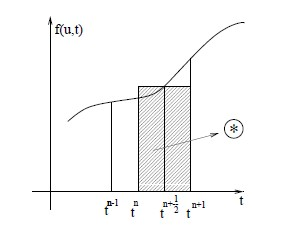
\includegraphics[height=0.6\textheight]{img/22/metoda_skokowa.jpg}
	\end{figure}
\end{frame}
%%%%%%%%%%%%%%%%%%%%%
\begin{frame}{Stabilność}
	$$\varepsilon^{n+1} = \varepsilon^n - \frac{\partial f}{\partial u}\bigg\arrowvert_n\Delta t\bigg[\frac{\partial f}{\partial u} \bigg\arrowvert_n\frac{\Delta t}{2}\bigg]\varepsilon^n$$
    $$g = 1-\alpha +\frac{1}{2}\alpha^2 \qquad \qquad \qquad \alpha = \frac{\partial f}{\partial u}\bigg\arrowvert_n \Delta t$$
    \newline
    - stabilna dla $\alpha$ rzeczywistego, gdy $\Delta t \leqslant \frac{2}{\frac{\partial f}{\partial u}\arrowvert_n}$
    \newline
    - może być niestabilna dla $\alpha$ urojonego
\end{frame}
%%%%%%%%%%%%%%%%%%%%%
